\section{System Design}
\label{sec:system-design}

\subsection{User Interface}
\label{sec:ui}

\begin{comment}
As argued in the previous section, user feedback is essential in determining, tracking and controlling the right hypothesis during the data exploration process.
With \system~we created a system that applies our heuristic automatically to all visualizations. We designed \system~'s user interface with a few goals in mind.

First, the user should be able to see the hypotheses the system assumed so far, their \pvals, effect sizes and if they are considered significant and should be able to change, add or delete hypotheses at any given stage of the exploration. 

Second, hypotheses rejection decisions should never change based on future user actions unless the user explicitly asks for it. We therefore require an incremental procedure to control the multiple hypothesis risk that does not change its rejection decisions even if more hypothesis tests are executed.
For example, the system should not state that their is a significant age difference for not married highly educated people, and then later on revoke its assessment just because the user did more tests. 
More formally, if the system determined which hypotheses $m_1 ...  m_n$ are significant (i.e., it rejects the null) or not and the user changes the last hypothesis or adds an hypothesis $m_{n+1}$, which should be the most common cases, the significance of hypotheses $m_1..m_{n}$ should not change. 
However, if the user might change, delete, or add hypothesis $k \in {1,..,n}$, depending on the used procedure we might allow that the significance of hypotheses $m_{k+1}$ to $m_n$ might have to change as well.
%Furthermore, the system automatically reports on the {\bf effect size} as a color coded value based on Cohen's suggestions \cite{something}.
%This is according to best practice, as the effect size (e.g., the age difference) determines how big the observed difference is compared to the variance. 

Third, individual hypothesis descriptions should be augmented with information about how much data $n^{H1}$ the user has to add, under the assumption that the new data will follow the current observed distribution of the data, to make an hypothesis significant. 
While sounding counter-intuitive, as one might (wrongly) imply, it is possible to make any hypothesis true by adding more data, calculating this value is in some fields already common practice. 
For example, in genetics scientist often search (automatically) for correlations between genes and high-level effects (like cancer). 
If such a correlation is found, often because of the multiple hypothesis error the chance of a true discovery is tiny (i.e., the \pval is too high). 
In that case the scientist works backwards and estimates how much more genes she has to to sequence in order to make the hypothesis relevant, expecting that the new data (e.g., gene sequences) follow the same distribution of the data the scientist already has.
However, if the effect was just produced by chance, the new data will be more similar to the distribution of the null-hypothesis and the null will not be rejected.  
%Similar, it is possible for a rejected null-hypothesis to calculate how much data $n^{H0}$ has to be added if the null-hypothesis is true, until the null-hypothesis will be accepted. 
% Eli: This has no statistical meaning.
The required value is generally easy to calculate or approximate,  and are highly valuable for the end-user. 
A small value for $n^{H1}$ in relation to the number of totally tested hypotheses might be an indication that the power (i.e., the chance to accept a true alternative hypothesis) of the test was not sufficiently large. 

And finally, users should be able to bookmark important hypotheses. 
Our system uses default hypothesis throughout the exploration and the user might find it too cumbersome to correct everyone for his real intentions, there might be more hypotheses generated than the user intended to test. 
Even if all hypotheses are what the user was considering, some of them might be more important to her than others; the hypotheses the user would like to include in a presentation or show to her boss. 
A key key question becomes, what is the expected number of false discoveries among those important discoveries?
\end{comment}

\begin{figure}
\centering
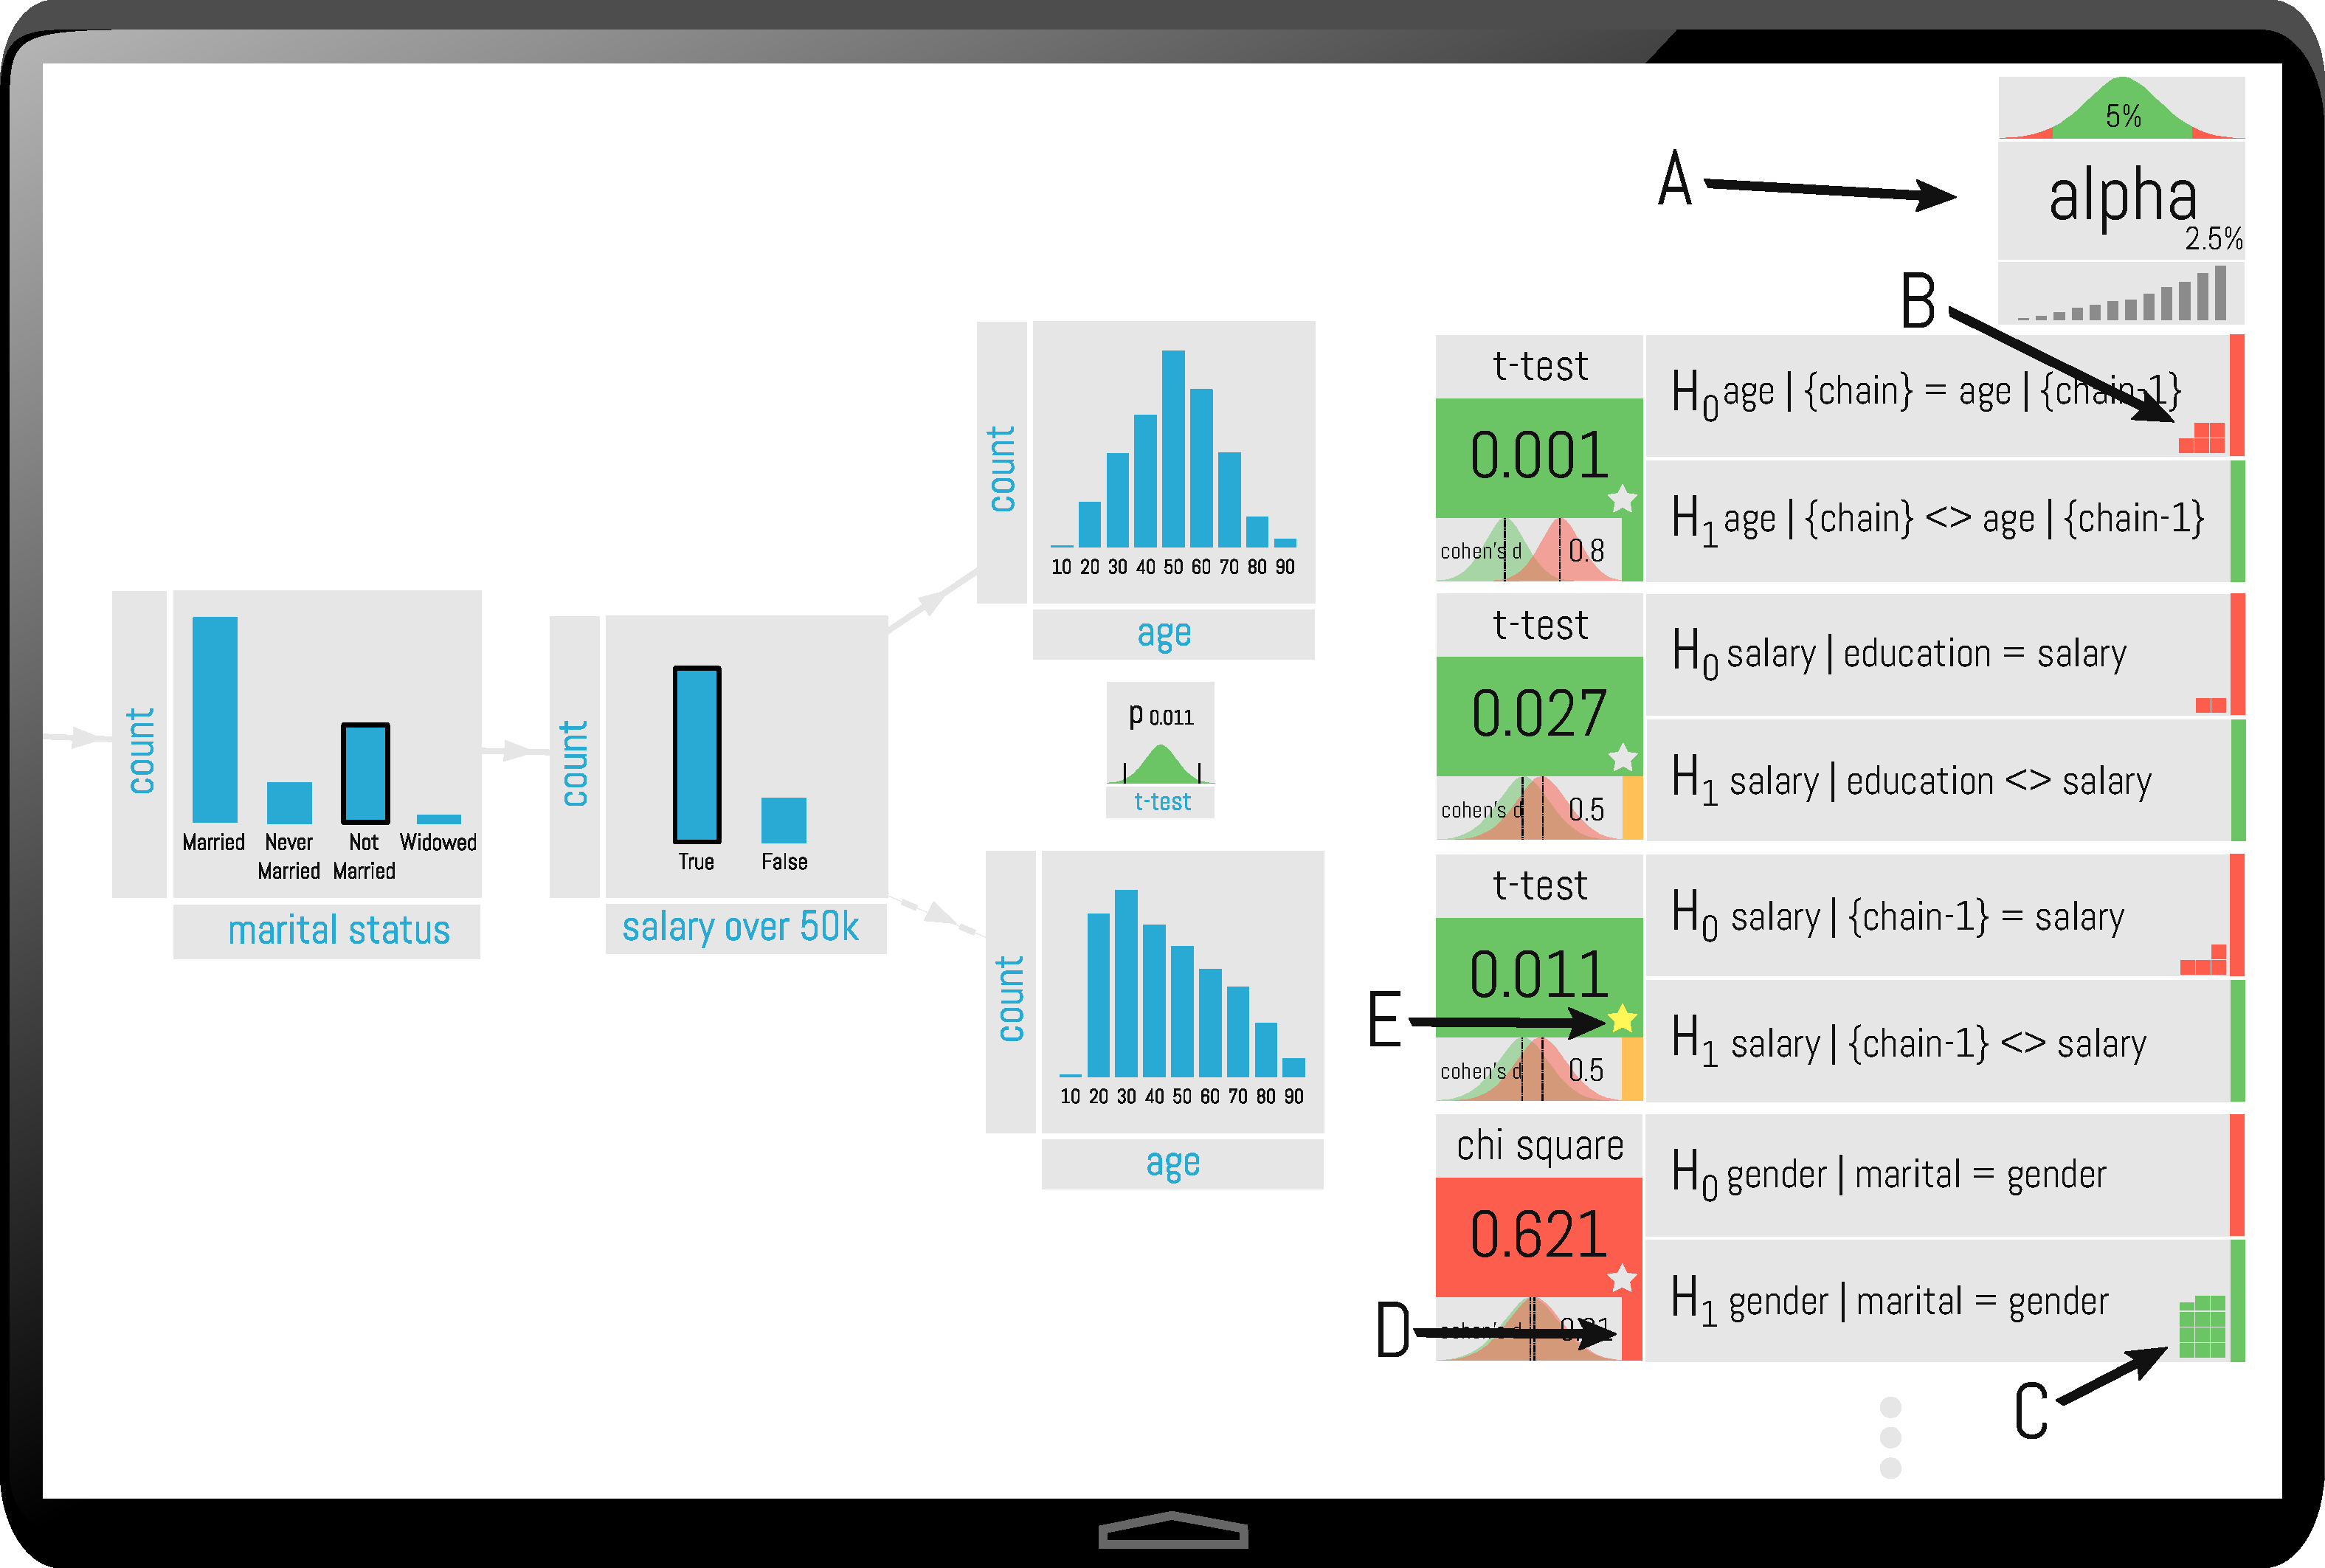
\includegraphics[width=0.48\textwidth]{figures/ui.pdf}
\caption{User Interface}
\label{fig:ui}	
\end{figure}

\sam{todo: how to let user specify hypotheses; remove (B); hypothesis re-test once data added; past hypothesis lookup/redraw}
The user interface of \system{} features an unbounded 2D canvas where visualizations can be laid out in a free form fashion (Figure~\ref{fig:ui}). A ``risk-gauge'' on the right-hand side of the display (Figure~\ref{fig:ui} (A)) serves two purposes, namely, to give user a summary of the control procedure (e.g., the budget for the false discovery rate set to 5\% with current remaining wealth of 2.5\% \sam{revisit this example}), and to provide access to a scrollable list of all the hypotheses that have been explored.
Each list entry displays details about an observation and its statistical significance.  

The text labels describe the null and alternative hypotheses concerning each observation and the corresponding hypothesis test and \pval. Each color coded tile indicates whether the observation is statistically significant or insignificant, which corresponds to green or red respectively.  The distributions of null and alternative hypotheses and the color coded effect size are also visualized (D).  To help the user understand the effect of data collection, the sample size estimate for the current significance level is displayed for each hypothesis test assuming the effect size is fixed (C).  For example, the five green squares in (C) indicates approximately five times the current data size with the same effect size would make this observation significant. Finally, important observations can be marked by tapping the ``star'' icons (E).

\subsection{Backend}
\label{sec:backend}

\begin{figure}
\centering
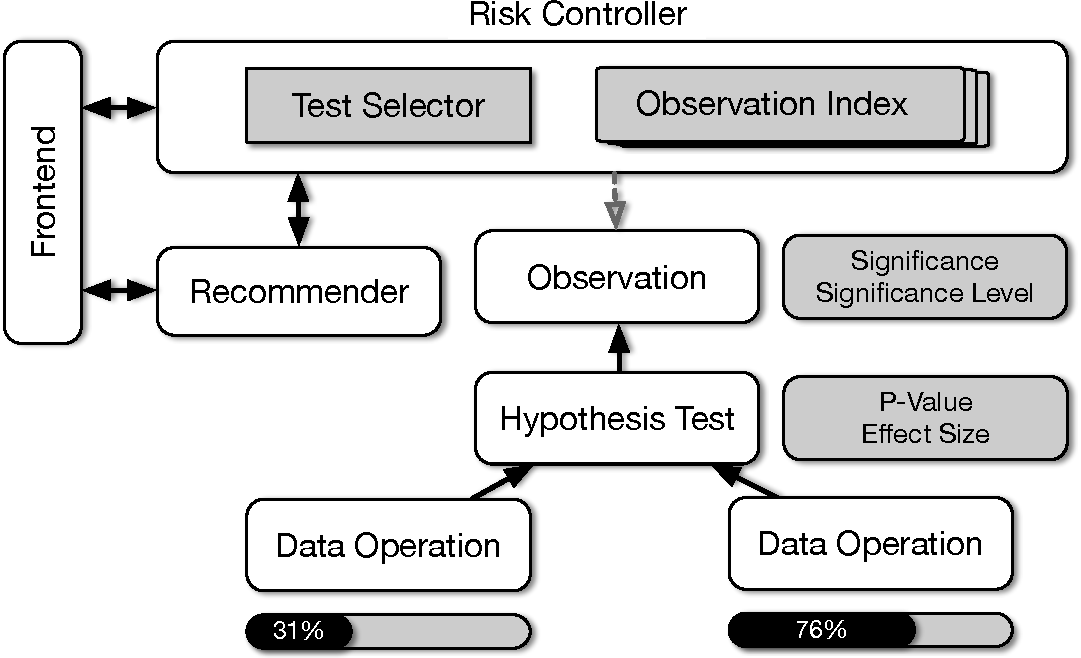
\includegraphics[scale=0.4]{figures/risk-controller.pdf}
\caption{Backend}
\label{fig:backend}	
\end{figure}

The highlight of the \system{} backend is the distributed and parallel computation of data-driven observations while preserving the linear ordering necessary for the false discovery procedures introduced in~\cite{zhao2016controlling}.  Our design combines functional reactive programming~\cite{wan2000functional} and progressive approximation paradigm~\cite{onlineagg,zgraggen2016progressive,vizdom} to dataflow processing to achieve interactivity and scalability.

The central piece of the \system{} backend is the risk controller that implements the false discovery control procedures as introduced in~\cite{zhao2016controlling}.  Figure~\ref{fig:backend} highlights the design.  A risk controller bootstraps with a predefined exploration ``budget'' on a new dataset and is ``invested'' on each observation.  Observations are created by either the frontend user manually or the backend recommender.  Observations are tracked and indexed by the risk controller to make global decisions on each observation's appropriate significance level and its significance. A loose analogy of the observation index is perhaps a version control system, such as Git~\cite{torvalds2010git}, but in this case for data-driven observations. Such design allows distributed and parallel computation of observations for better performance, yet meanwhile enforces a linear ordering for the false discovery control procedures in~\cite{zhao2016controlling}. The observation index can also be used to look up the same observations for different frontend users or the backend recommender. 

\system{} composes operations into dataflow.  For example, an observation depends on its underlying hypothesis test, which then depends on the data operations.  An observation is a comparison of two distributions based on different conditions.  A comparison, for example, can be of the means, variances, correlations or histogram frequencies. Each observation is formulated as a null and an alternative hypothesis.  The risk controller is responsible of choosing the appropriate hypothesis test based on a given observation.  For example, to compare two means being different, a two-sided $t$-test is chosen.  $\chi^2$-test is used to compare two histograms, but only when the frequencies are large enough. For small frequencies, a permutation test is used. 

An data operation, on the other hand, extracts information from the underlying data source.  For example, an ``EmpiricalDistOperation'' calculates the mean and variance on the given attribute; whereas a ``HistogramOperation'' constructs bins and frequencies from some attribute.  Filters are pushed down to data operations.

\system{} implements the reactive programming~\cite{wan2000functional} and progressive approximation paradigm~\cite{vizdom, zgraggen2016progressive}. Operations constitute a dataflow graph that is reactive, where approximate updates are pushed as a stream from observed to observer operations. Data operations computes approximate information about the data source based on sampling, which eventually converges to the exact information as it completes the pass on the data source. The approximate information then forms an update stream that is pushed to any relevant hypothesis tests. A hypothesis test observes the approximate updates to calculate the effect sizes and \pvals, which in turn serve as the input to the risk controller to determine the significance of the observation progressively. 

Data updates necessitates the risk controller to re-evaluate the affected observations. Observations can be affected by two aspects of data updates, where the observed data is changed such that certain observation becomes significant or insignificant, or some earlier observation with changed significance affects the later observations.  Analogous to a database recovery algorithm such as ARIES~\cite{mohan1992aries}, the risk controller will first recover its exploration budget and then automatically ``redo'' the observations through the observation index.  The optimization is to minimize the re-run of data operations.  The redo algorithm works in two phases.  It first collects all data-affected observations whose underlying data operations overlap with the updated data.  It then resets the exploration budget to that of the first data-affected observations, and updates the underlying hypothesis tests by re-running the data operations.  Otherwise the redo algorithm only updates the significance level and significance for the other affected observations.